\documentclass[15pt,serif,mathserif,final]{beamer}
\mode<presentation>{\usetheme{Lankton}}
\usepackage{amsmath,amsfonts,amssymb,pxfonts,eulervm,xspace}
\usepackage{graphicx}
\usepackage{algorithm}
\usepackage{algorithmic}
\usepackage{tikz}
\usepackage{fancybox}
\usetikzlibrary{bayesnet}
\tikzstyle{connect}=[-latex]
\tikzstyle{allconnected}=[line width=0.1cm]



\graphicspath{{./}{../../../bo_stepsahead/reports/diagrams/}}
\newcommand{\todiagrams}{../diagrams/}
\usepackage[orientation=portrait,size=custom,width=70,height=40,scale=.6,debug]{beamerposter}
%\usepackage{xspace}

%\newcommand{\acr}[1]{\textsc{#1}\xspace}
%\newcommand{\gp}{\acr{gp}}
%\newcommand{\dpp}{\acr{dpp}}
%\newcommand{\us}{\acr{glasses}}
%\newcommand{\direct}{\acr{direct}}
%\newcommand{\lbfgs}{\acr{l-bfgs}}
%\newcommand{\map}{\acr{map}}
%\newcommand{\ep}{\acr{ep}}
%\newcommand{\bo}{\acr{bo}}
%\newcommand{\mpi}{\acr{mpi}}
%\newcommand{\el}{\acr{el}}
%\newcommand{\lcb}{\acr{gp-lcb}}


\newcommand{\vp}{\vec{\phi}}
\newcommand{\vmu}{\vec{\mu}}
\newcommand{\vf}{\vec{f}}
\newcommand{\I}{\mathcal{I}}
\newcommand{\ud}{\mathrm{d}}
\newcommand{\E}{\mathbb{E}}
%\newcommand{\dataVector}{\textbf{y}}
\newcommand{\bL}{\textbf{L}}
\newcommand{\bI}{\textbf{I}}
\newcommand{\vk}{\vec{k}}
\newcommand{\vL}{\vec{\Lambda}}
\newcommand{\xmin}{x_{\min}}
\newcommand{\pmin}{p_{\min}}
\newcommand{\fmin}{f_{\min}}
\newcommand{\pfmin}{p_{f_{\min}}}
\renewcommand{\vec}{\boldsymbol}
\newcommand{\fun}[1]{\mathsf{#1}}
\renewcommand{\O}{\mathcal{O}}
\newcommand{\GP}{\mathcal{GP}}
\newcommand{\N}{\mathcal{N}}
\newcommand{\Id}{\vec{I}}
\newcommand{\II}{\mathbb{I}}
\newcommand{\future}{\mathcal{F}}
\newcommand{\IR}{\mathbb{R}}
\newcommand{\argmin}{\operatorname*{arg\: min}}
\newcommand{\argmax}{\operatorname*{arg\: max}}
\newcommand{\chol}{\operatorname{\mathsf{C}}}

\newcommand{\xst}{x_{\ast}}
\newcommand{\yst}{y_{\ast}}


\graphicspath{{../diagrams/}}
% This file defines notation to be used
\global\long\def\outputIndex{j}
\global\long\def\dataIndex{i}
\global\long\def\dataIndexTwo{j}
\global\long\def\latentIndex{j}

\global\long\def\inputSpace{\mathcal{X}}

\global\long\def\conditionalCovariance{\boldsymbol{\Sigma}}

\global\long\def\fantasyDim{r}
\global\long\def\dataDim{p}
\global\long\def\latentDim{q}
\global\long\def\inputDim{q}
\global\long\def\numLayers{\ell}
\global\long\def\numData{n}
\global\long\def\numTime{T}
\global\long\def\numTasks{m}
\global\long\def\numSequences{s}
\global\long\def\numInducing{m}
\global\long\def\numNeighbors{K}
\global\long\def\numHidden{h}
\global\long\def\numComponents{m}
\global\long\def\numBasisFunc{m}
\global\long\def\iterNum{k}
\global\long\def\maxIters{K}

\global\long\def\rbfWidth{\ell}
\global\long\def\lengthScale{\ell}
\global\long\def\binomProb{\pi}

\global\long\def\dataStd{\sigma}
\global\long\def\featureStd{\varsigma}

\global\long\def\heaviside{H}
\global\long\def\errorFunction{E}
\global\long\def\likelihoodFunction{L}
\global\long\def\likelihoodBound{\mathcal{L}}
\global\long\def\lagrangian{L}

\global\long\def\parameterScalar{\theta}
\global\long\def\parameterVector{\boldsymbol{\parameterScalar}}
\global\long\def\parameterMatrix{\boldsymbol{\Theta}}

\global\long\def\dataScalar{y}
\global\long\def\dataVector{\mathbf{\dataScalar}}
\global\long\def\dataMatrix{\mathbf{\MakeUppercase{\dataScalar}}}

\global\long\def\cdataMatrix{\hat{\dataMatrix}}
\global\long\def\cdataVector{\hat{\dataVector}}
\global\long\def\cdataScalar{\hat{\dataScalar}}

\global\long\def\dataSet{\mathcal{D}}

\global\long\def\bigO{\mathcal{O}}


\global\long\def\switchScalar{s}
\global\long\def\switchVector{\mathbf{\switchScalar}}
\global\long\def\switchMatrix{\mathbf{\MakeUppercase{\switchScalar}}}

\global\long\def\latentScalar{x}
\global\long\def\latentMatrix{\mathbf{\MakeUppercase{\latentScalar}}}
\global\long\def\latentVector{\mathbf{\latentScalar}}

\global\long\def\hiddenScalar{h}
\global\long\def\hiddenMatrix{\mathbf{\MakeUppercase{\hiddenScalar}}}
\global\long\def\hiddenVector{\mathbf{\hiddenScalar}}

\global\long\def\noiseMatrix{\boldsymbol{E}}
\global\long\def\noiseVector{\boldsymbol{\epsilon}}
\global\long\def\noiseScalar{\epsilon}

\global\long\def\fantasyScalar{z}
\global\long\def\fantasyVector{\mathbf{\fantasyScalar}}
\global\long\def\fantasyMatrix{\mathbf{\MakeUppercase{\fantasyScalar}}}

\global\long\def\kernelScalar{k}
\global\long\def\kernelVector{\mathbf{\kernelScalar}}
\global\long\def\kernelMatrix{\mathbf{\MakeUppercase{\kernelScalar}}}

\global\long\def\centeredKernelScalar{b}
\global\long\def\centeredKernelVector{\centeredKernelScalar}
\global\long\def\centeredKernelMatrix{\mathbf{\MakeUppercase{\centeredKernelScalar}}}

\global\long\def\latentForce{f}
\global\long\def\LatentForce{F}
\global\long\def\displacement{x}
\global\long\def\displacementVector{\textbf{\displacement}}
\global\long\def\Displacement{X}
\global\long\def\velocity{v}
\global\long\def\acceleration{a}
\global\long\def\lengthScale{\ell}
\global\long\def\naturalFrequency{\omega}
\global\long\def\sensitivity{s}
\global\long\def\mrnaConcentration{m}
\global\long\def\tfConcentration{p}
\global\long\def\tfMrnaConcentration{f}
\global\long\def\tfVector{{\bf \tfConcentration}}
\global\long\def\weightScalar{w}
\global\long\def\weightVector{{\bf \weightScalar}}
\global\long\def\meanVector{\boldsymbol{\mu}}
\global\long\def\zerosVector{{\bf 0}}
\global\long\def\decayRate{d}
\global\long\def\dampingCoefficient{c}
\global\long\def\mass{m}
\global\long\def\basalRate{b}
\global\long\def\Sensitivity{S}
\global\long\def\DecayRate{D}
\global\long\def\tfDecayRate{\delta}
\global\long\def\DampingCoefficient{C}
\global\long\def\Mass{M}
\global\long\def\BasalRate{B}
\global\long\def\basisFunc{\phi}
\global\long\def\basisFuncVector{\boldsymbol{\basisFunc}}
\global\long\def\numBasisFunc{m}
\global\long\def\numData{n}
\global\long\def\numComps{K}
\global\long\def\dataDim{p}

\global\long\def\inputScalar{x}
\global\long\def\inputMatrix{{\bf \MakeUppercase{\inputScalar}}}
\global\long\def\inputVector{{\bf \inputScalar}}

\global\long\def\parameterScalar{\theta}
\global\long\def\parameterVector{\boldsymbol{\parameterScalar}}

\global\long\def\kernel{\kernelScalar}

\global\long\def\covarianceScalar{c}
\global\long\def\covarianceMatrix{\mathbf{\MakeUppercase{\covarianceScalar}}}
\global\long\def\covarianceVector{\mathbf{\covarianceScalar}}

\global\long\def\croupierScalar{s}
\global\long\def\croupierMatrix{\mathbf{\MakeUppercase{\croupierScalar}}}
\global\long\def\croupierVector{\mathbf{\croupierScalar}}

\global\long\def\coregionalizationScalar{b}
\global\long\def\coregionalizationMatrix{\mathbf{\MakeUppercase{\coregionalizationScalar}}}
\global\long\def\coregionalizationVector{\mathbf{\coregionalizationScalar}}

\global\long\def\precisionScalar{j}
\global\long\def\precisionMatrix{\mathbf{\MakeUppercase{\precisionScalar}}}
\global\long\def\precisionVector{\mathbf{\precisionScalar}}

\global\long\def\meanScalar{\mu}
\global\long\def\meanMatrix{\mathbf{M}}
\global\long\def\meanVector{\boldsymbol{\meanScalar}}

\global\long\def\meanTwoScalar{m}
\global\long\def\meanTwoVector{\mathbf{\meanTwoScalar}}
\global\long\def\meanTwoMatrix{\mathbf{\MakeUppercase{\meanTwoScalar}}}

\global\long\def\locationScalar{\mu}
\global\long\def\locationMatrix{\mathbf{M}}
\global\long\def\locationVector{\boldsymbol{\locationScalar}}

\global\long\def\eigenvectorScalar{u}
\global\long\def\eigenvector{\mathbf{\eigenvectorScalar}}
\global\long\def\eigenvectorMatrix{\mathbf{\MakeUppercase{\eigenvectorScalar}}}

\global\long\def\eigenvalue{\lambda}
\global\long\def\eigenvalueVector{\boldsymbol{\lambda}}
\global\long\def\eigenvalueMatrix{\boldsymbol{\Lambda}}

\global\long\def\singularvalue{\ell}
\global\long\def\singularvalueVector{\mathbf{l}}
\global\long\def\singularvalueMatrix{\mathbf{L}}

\global\long\def\eigenvectwoScalar{v}
\global\long\def\eigenvectwo{\mathbf{v}}
\global\long\def\eigenvectwoMatrix{\mathbf{V}}

\global\long\def\eigenvaltwo{\ell}
\global\long\def\eigenvaltwoVector{\mathbf{l}}
\global\long\def\eigenvaltwoMatrix{\mathbf{L}}

\global\long\def\laplacianScalar{\ell}
\global\long\def\laplacianVector{\mathbf{\ell}}
\global\long\def\laplacianMatrix{\mathbf{L}}

\global\long\def\normalizedLaplacianScalar{\hat{\ell}}
\global\long\def\normalizedLaplacianVector{\hat{\mathbf{\ell}}}
\global\long\def\normalizedLaplacianMatrix{\hat{\mathbf{L}}}

\global\long\def\weightedAdjacencyScalar{a}
\global\long\def\weightedAdjacencyVector{\mathbf{\weightedAdjacencyScalar}}
\global\long\def\weightedAdjacencyMatrix{\mathbf{\MakeUppercase{\weightedAdjacencyScalar}}}


\global\long\def\degreeScalar{d}
\global\long\def\degreeVector{\mathbf{\degreeScalar}}
\global\long\def\degreeMatrix{\mathbf{\MakeUppercase{\degreeScalar}}}

\global\long\def\lagrangeMultiplier{\lambda}
\global\long\def\lagrangeMultiplierMatrix{\boldsymbol{\Lambda}}

\global\long\def\laplacianFactor{\mathbf{\MakeUppercase{\laplacianFactorScalar}}}
\global\long\def\laplacianFactorScalar{m}
\global\long\def\laplacianFactorVector{\mathbf{\laplacianFactorScalar}}

\global\long\def\sufficientStatsScalar{g}
\global\long\def\sufficientStatsVector{\mathbf{\sufficientStatsScalar}}
\global\long\def\sufficientStatsMatrix{\mathbf{\MakeUppercase{\sufficientStatsScalar}}}

\global\long\def\mappingScalar{w}
\global\long\def\mappingVector{\mathbf{\mappingScalar}}
\global\long\def\mappingMatrix{\mathbf{W}}

\global\long\def\mappingScalarTwo{v}
\global\long\def\mappingVectorTwo{\mathbf{\mappingScalarTwo}}
\global\long\def\mappingMatrixTwo{\mathbf{\MakeUppercase{\mappingScalarTwo}}}

\global\long\def\responsibility{r}

\global\long\def\mappingFunction{f}
\global\long\def\mappingFunctionVector{\mathbf{\mappingFunction}}
\global\long\def\mappingFunctionMatrix{\mathbf{\MakeUppercase{\mappingFunction}}}
\global\long\def\mappingFunctionTwo{g}
\global\long\def\mappingFunctionTwoVector{\mathbf{\mappingFunctionTwo}}
\global\long\def\mappingFunctionTwoMatrix{\mathbf{\MakeUppercase{\mappingFunctionTwo}}}

\global\long\def\pseudotargetScalar{u}
%\global\long\def\pseudotargetScalar{\widetilde{y}}
\global\long\def\pseudotargetVector{\mathbf{\pseudotargetScalar}}
\global\long\def\pseudotargetMatrix{\mathbf{\MakeUppercase{\pseudotargetScalar}}}

\global\long\def\inducingScalar{u}
\global\long\def\inducingVector{\mathbf{\inducingScalar}}
\global\long\def\inducingMatrix{\mathbf{\MakeUppercase{\inducingScalar}}}

\global\long\def\inducingInputScalar{z}
\global\long\def\inducingInputVector{\mathbf{\inducingInputScalar}}
\global\long\def\inducingInputMatrix{\mathbf{\MakeUppercase{\inducingInputScalar}}}

\global\long\def\latentFunction{u}
\global\long\def\latentFunctionVector{\mathbf{\latentFunction}}
\global\long\def\latentFunctionMatrix{\mathbf{\MakeUppercase{\latentFunction}}}

\global\long\def\basisFunc{\phi}
\global\long\def\basisFunction{\phi}
\global\long\def\basisVector{\boldsymbol{\basisFunction}}
\global\long\def\basisScalar{\basisFunction}
\global\long\def\basisLocation{\mu}
\global\long\def\basisMatrix{\boldsymbol{\Phi}}
\global\long\def\cbasisMatrix{\hat{\boldsymbol{\Phi}}}

\global\long\def\numFeatures{K}
\global\long\def\numActive{m}

\global\long\def\paramVector{\boldsymbol{\theta}}

\global\long\def\expectedDistanceMatrix{\mathcal{D}}

\global\long\def\latentDistanceScalar{\delta}
\global\long\def\latentDistanceVector{\boldsymbol{\delta}}
\global\long\def\latentDistanceMatrix{\boldsymbol{\Delta}}

\global\long\def\springScalar{\kappa}
\global\long\def\springVector{\boldsymbol{\kappa}}
\global\long\def\springMatrix{\boldsymbol{\mathcal{K}}}

\global\long\def\mrnaConcentration{m}
\global\long\def\decayRate{d}
\global\long\def\basalRate{b}
\global\long\def\sensitivity{s}
\global\long\def\learnRate{\eta}

\global\long\def\distanceScalar{d}
\global\long\def\distanceVector{\mathbf{\distanceScalar}}
\global\long\def\distanceMatrix{\mathbf{\MakeUppercase{\distanceScalar}}}


\global\long\def\bScalar{b}
\global\long\def\bVector{\mathbf{b}}
\global\long\def\bMatrix{\mathbf{B}}

\global\long\def\Amatrix{\mathbf{A}}

\global\long\def\weightScalar{w}
\global\long\def\weightVector{\mathbf{\weightScalar}}
\global\long\def\weightMatrix{\mathbf{\MakeUppercase{\weightScalar}}}

\global\long\def\vScalar{v}
\global\long\def\vVector{\mathbf{v}}
\global\long\def\vMatrix{\mathbf{V}}

\global\long\def\cMatrix{\mathbf{C}}

\global\long\def\aMatrix{\mathbf{A}}
\global\long\def\aVector{\mathbf{a}}
\global\long\def\aScalar{a}

\global\long\def\centeringMatrix{\mathbf{H}}

\global\long\def\eye{\mathbf{I}}
\global\long\def\identityMatrix{\eye}
\global\long\def\onesVector{\mathbf{1}}
\global\long\def\zerosVector{\mathbf{0}}
\global\long\def\half{\frac{1}{2}}



\global\long\def\numTrials{S}
\global\long\def\numSuccess{s}


\global\long\def\sampleCovScalar{s}
\global\long\def\sampleCovVector{\mathbf{\sampleCovScalar}}
\global\long\def\sampleCovMatrix{\mathbf{\MakeUppercase{\sampleCovScalar}}}

\global\long\def\rotationScalar{r}
\global\long\def\rotationVector{\mathbf{\rotationScalar}}
\global\long\def\rotationMatrix{\mathbf{\MakeUppercase{\rotationScalar}}}

\global\long\def\diff#1#2{\frac{\text{d}#1}{\text{d}#2}}
\global\long\def\partDiff#1#2{\frac{\partial#1}{\partial#2}}
\global\long\def\inlineDiff#1#2{\text{d}#1/\text{d}#2}
\global\long\def\diffTwo#1#2{\frac{\text{d}^2#1}{\text{d}#2^2}}

\global\long\def\gaussianSamp#1#2{\mathcal{N}\left(#1,#2\right)}
\global\long\def\gaussianDist#1#2#3{\mathcal{N}\left(#1|#2,#3\right)}
\global\long\def\rayleighDist#1#2{\mathcal{R}\left(#1|#2\right)}
\global\long\def\rayleighSamp#1{\mathcal{R}\left(#1\right)}

\global\long\def\entropy#1{\mathcal{H}\left(#1\right)}


\global\long\def\gammaSamp#1#2{\mathcal{G}\left(#1,#2\right)}
\global\long\def\gammaDist#1#2#3{\mathcal{G}\left(#1|#2,#3\right)}
\global\long\def\gammaCdf#1#2#3{\mathcal{GAMMA CDF}\left(#1|#2,#3\right)}

\global\long\def\expSamp#1{\left<#1\right>}
\global\long\def\expDist#1#2{\left<#1\right>_{#2}}

\global\long\def\covSamp#1{\text{cov}\left(#1\right)}
\global\long\def\covDist#1#2{\text{cov}_{#2}\left(#1\right)}

\global\long\def\variance#1{\text{var}\left( #1 \right)}
\global\long\def\varianceDist#1#2{\text{var}_{#2}\left( #1 \right)}

\global\long\def\chiSquaredSamp#1{\chi_{#1}^{2}}
\global\long\def\chiSquaredDist#1#2{\chi_{#1}^{2}\left(#2\right)}

\global\long\def\diagonalMatrix{\mathbf{D}}

\global\long\def\spar{\lambda}
\global\long\def\sorth{\mathbf{u}}

\global\long\def\expectation#1{\left\langle #1 \right\rangle }
\global\long\def\expectationDist#1#2{\left\langle #1 \right\rangle _{#2}}

\global\long\def\KL#1#2{\text{KL}\left( #1\,\|\,#2 \right)}



\global\long\def\kff{\kernelScalar_{\mappingFunction \mappingFunction}}
\global\long\def\kfu{\kernelVector_{\mappingFunction \inducingScalar}}
\global\long\def\kuf{\kernelVector_{\inducingScalar \mappingFunction}}
\global\long\def\kuu{\kernelVector_{\inducingScalar \inducingScalar}}

\global\long\def\Kff{\kernelMatrix_{\mappingFunctionVector \mappingFunctionVector}}
\global\long\def\Kuu{\kernelMatrix_{\inducingVector \inducingVector}}
\global\long\def\Kuui{\Kuu^{-1}}
\global\long\def\Kastu{\kernelMatrix_{\mathbf{\ast} \inducingVector}}
\global\long\def\Kuast{\kernelMatrix_{\inducingVector \bf\ast}}
\global\long\def\Kaast{\kernelMatrix_{\mathbf{ \ast}\mathbf{ \ast}}}
\global\long\def\Qaast{{\bf Q}_{\bf \ast \ast}}
\global\long\def\Qfast{{\bf Q}_{\mappingFunctionVector \bf \ast}}
\global\long\def\Qastf{{\bf Q}_{\ast \mappingFunction}}
\global\long\def\Kfu{\kernelMatrix_{\mappingFunctionVector \inducingVector}}
\global\long\def\Kuf{\kernelMatrix_{\inducingVector \mappingFunctionVector}}
\global\long\def\Qff{{\bf Q}_{\mappingFunctionVector \mappingFunctionVector}}

\global\long\def\det#1{\left|#1\right|}
\global\long\def\rank#1{\text{rank}\left(#1\right)}
\global\long\def\vec#1{#1:}
\global\long\def\vecb#1{\left(#1\right):}
\global\long\def\tr#1{\text{tr}\left(#1\right)}
\global\long\def\diag#1{\text{diag}\left(#1\right)}
\global\long\def\sign#1{\text{sign}\left(#1\right)}
\global\long\def\twonorm#1{\left\vert#1\right\vert_2}
\global\long\def\onenorm#1{\left\vert#1\right\vert_1}
\global\long\def\twonorm#1{\left\Vert #1 \right\Vert}
%\global\long\def\norm#1#2{\left\Vert #1 \right\Vert_{#2}}
\global\long\def\neighborhood#1{\mathcal{N}\left( #1 \right)}
\global\long\def\ltwoNorm#1{\left\Vert #1 \right\Vert_2}
\global\long\def\norm#1{\left\Vert #1 \right\Vert}
\global\long\def\loneNorm#1{\left\Vert #1 \right\Vert_1}
\global\long\def\scalarProduct#1#2{\left\langle{#1},{#2}\right\rangle}



% This file defines macros, notation is defined in notationDef.tex
\usepackage{color}
\usepackage{verbatim}

\global\long\def\neil#1{\textbf{\color{red}#1}}
%\global\long\def\todo#1{\textbf{TODO: #1}}
\global\long\def\instructions#1{\textbf{INSTRUCTIONS: #1}}

\definecolor{brown}{rgb}{0.9,0.59,0.078}
\definecolor{ironsulf}{rgb}{0,0.7,.5}
\definecolor{lightpurple}{rgb}{0.156,0,0.245}

\newenvironment{matlab}{\comment}{\endcomment}
\newenvironment{octave}{\comment}{\endcomment}
\newenvironment{matlabv}{\verbatim}{\endverbatim}
\newenvironment{octavev}{\verbatim}{\endverbatim}

\ifdefined\blackBackground
\definecolor{colorOne}{rgb}{0, 1, 1}
\definecolor{colorTwo}{rgb}{1, 0, 1}
\definecolor{colorThree}{rgb}{1, 1, 0}
\definecolor{colorTwoThree}{rgb}{1, 0, 0}
\definecolor{colorOneThree}{rgb}{0, 1, 0}
\definecolor{colorOneTwo}{rgb}{0, 0, 1}
\else
\definecolor{colorOne}{rgb}{1, 0, 0}
\definecolor{colorTwo}{rgb}{0, 1, 0}
\definecolor{colorThree}{rgb}{0, 0, 1}
\definecolor{colorTwoThree}{rgb}{0, 1, 1}
\definecolor{colorOneThree}{rgb}{1, 0, 1}
\definecolor{colorOneTwo}{rgb}{1, 1, 0}
\fi

\ifdefined\blackBackground
\global\long\def\redColor{cyan}
\global\long\def\greenColor{magenta}
\global\long\def\blueColor{yellow}
\global\long\def\magentaColor{green}
\global\long\def\blackColor{white}
\global\long\def\whiteColor{black}
\else
\global\long\def\redColor{red}
\global\long\def\greenColor{green}
\global\long\def\blueColor{blue}
\global\long\def\magentaColor{magenta}
\global\long\def\blackColor{black}
\global\long\def\whiteColor{white}
\fi

\global\long\def\det#1{\left|#1\right|}
\global\long\def\erf{\text{erf}}
\global\long\def\refeq#1{(\ref{#1})}
\global\long\def\refsec#1{Section \ref{#1}}
\global\long\def\refsecs#1#2{Sections \ref{#1}--\ref{#2}}
\global\long\def\reftwosec#1#2{Sections \ref{#1} and \ref{#2}}
\global\long\def\Refsec#1{Section \ref{#1}}

% Try and avoid these macros for notation, they are definitions of convenience.
\global\long\def\bfdelta{\boldsymbol{\delta}}
\global\long\def\bfDelta{\boldsymbol{\Delta}}
\global\long\def\bfbeta{\boldsymbol{\beta}}
\global\long\def\bfgamma{\boldsymbol{\gamma}}
\global\long\def\bfmu{\boldsymbol{\mu}}
\global\long\def\bfnu{\boldsymbol{\nu}}
\global\long\def\bfalpha{\boldsymbol{\alpha}}
\global\long\def\bfepsilon{\boldsymbol{\epsilon}}
\global\long\def\bfSigma{\boldsymbol{\Sigma}}
\global\long\def\bftau{\boldsymbol{\tau}}
\global\long\def\bflambda{\boldsymbol{\lambda}}
\global\long\def\bfLambda{\boldsymbol{\Lambda}}
\global\long\def\bfpsi{\boldsymbol{\psi}}
\global\long\def\bfxi{\boldsymbol{\xi}}
\global\long\def\bfpi{\bm{\pi}}
\global\long\def\bfPsi{\boldsymbol{\Psi}}
\global\long\def\bfphi{\boldsymbol{\phi}}
\global\long\def\bfPhi{\boldsymbol{\Phi}}
\global\long\def\bfrho{\boldsymbol{\rho}}
\global\long\def\bftheta{\boldsymbol{\theta}}
\global\long\def\bfTheta{\boldsymbol{\Theta}}
\global\long\def\bfomega{\boldsymbol{\omega}}


\global\long\def\Bmath#1{\boldsymbol{#1}}


% Avoid these macros for notation, they are definitions of convenience.
\global\long\def\bfa{\mathbf{a}}
\global\long\def\bfb{\mathbf{b}}
\global\long\def\bfc{\mathbf{c}}
\global\long\def\bfd{\mathbf{d}}
\global\long\def\bfe{\mathbf{e}}
\global\long\def\bff{\mathbf{f}}
\global\long\def\bfg{\mathbf{g}}
\global\long\def\bfh{\mathbf{h}}
\global\long\def\bfk{\mathbf{k}}
\global\long\def\bfl{\mathbf{l}}
\global\long\def\bfm{\mathbf{m}}
\global\long\def\bfn{\mathbf{n}}
\global\long\def\bfo{\mathbf{o}}
\global\long\def\bfp{\mathbf{p}}
\global\long\def\bfq{\mathbf{q}}
\global\long\def\bfr{\mathbf{r}}
\global\long\def\bfs{\mathbf{s}}
\global\long\def\bft{\mathbf{t}}
\global\long\def\bfu{\mathbf{u}}
\global\long\def\bfv{\mathbf{v}}
\global\long\def\bfw{\mathbf{w}}
\global\long\def\bfx{\mathbf{x}}
\global\long\def\bfy{\mathbf{y}}
\global\long\def\bfz{\mathbf{z}}

\newcommand{\dif}[1]{\text{d}#1}
\global\long\def\cov{\text{cov}}


\global\long\def\bfzero{\mathbf{0}}
\global\long\def\bfone{\mathbf{1}}


\global\long\def\bfA{\mathbf{A}}
\global\long\def\bfB{\mathbf{B}}
\global\long\def\bfC{\mathbf{C}}
\global\long\def\bfD{\mathbf{D}}
\global\long\def\bfE{\mathbf{E}}
\global\long\def\bfG{\mathbf{G}}
\global\long\def\bfH{\mathbf{H}}
\global\long\def\bfI{\mathbf{I}}
\global\long\def\eye{\mathbf{I}}
\global\long\def\bfK{\mathbf{K}}
\global\long\def\bfL{\mathbf{L}}
\global\long\def\bfM{\mathbf{M}}
\global\long\def\bfO{\mathbf{O}}
\global\long\def\bfP{\mathbf{P}}
\global\long\def\bfQ{\mathbf{Q}}
\global\long\def\bfR{\mathbf{R}}
\global\long\def\bfS{\mathbf{S}}
\global\long\def\bfT{\mathbf{T}}
\global\long\def\bfU{\mathbf{U}}
\global\long\def\bfV{\mathbf{V}}
\global\long\def\bfW{\mathbf{W}}
\global\long\def\bfX{\mathbf{X}}
\global\long\def\bfY{\mathbf{Y}}
\global\long\def\bfZ{\mathbf{Z}}
\global\long\def\llangle{{\langle\vspace{-2mm} \langle}}
\global\long\def\rrangle{{\rangle\vspace{-2mm} \rangle}}
\global\long\def\la{\leftarrow}


\global\long\def\tf{\tilde{f}}
\global\long\def\tg{\tilde{g}}
\global\long\def\tX{\tilde{X}}
\global\long\def\tY{\tilde{Y}}
\global\long\def\tZ{\tilde{Z}}


\global\long\def\bbE{\mathbb{E}}
\global\long\def\bbR{\mathbb{R}}
\global\long\def\bbP{\mathbb{P}}
\global\long\def\bbT{\mathbb{T}}
\global\long\def\bbZ{\mathbb{Z}}


\global\long\def\ois{2 \pi i s}
\global\long\def\oik{2 \pi i k}
\global\long\def\oin{2 \pi i n}
\global\long\def\oim{2 \pi i m}


\global\long\def\T{{\top}}
\global\long\def\Tr{\mbox{Tr}}
\global\long\def\trace#1{\text{tr}\left(#1\right)}
%\global\long\def\diff#1{{\, d#1}}
\global\long\def\diff#1#2{\frac{\text{d}#1}{\text{d}#2}}
\global\long\def\vgraph#1{ \newpage\begin{center} \end{center}{center}{center}{center}{center}{center}{center}{center}{center}{center}{center}{center}{center}{center}{center}{center}{center} {\large{\bf #1}} {center} \vspace{2mm} }
\global\long\def\high#1{\textcolor{blue}{\emph{#1}}}
\global\long\def\cut#1{}
\global\long\def\citeasnoun#1{\citeN{#1}}
\global\long\def\citemulti#1#2{(#1, \citeyearNP{#2})}
\global\long\def\citemultiN#1#2{#1 (\citeyearNP{#2})}
\global\long\def\Sum{{\displaystyle \sum}}
\global\long\def\defeq{{\stackrel{def}{=}}}
\global\long\def\marg#1{\marginpar{#1}}


\global\long\def\pdt#1#2{\frac{\partial^{2} #1}{\partial{#2}^{2} }}
\global\long\def\pdsd#1#2#3{\frac{\partial^{2} #1}{\partial{#2} \partial{#3} }}
\global\long\def\pdo#1#2{\frac{\partial{#1}}{\partial{#2}}}
\global\long\def\pdol#1#2{\partial{#1}/ \partial{#2}}
\global\long\def\pdu#1{\frac{\partial}{\partial{#1}}}

\global\long\def\reffig#1{figure~\ref{#1}}
\global\long\def\Reffig#1{Figure~\ref{#1}}
\global\long\def\reffigrange#1#2{figure~\ref{#1}--\ref{#2}}
\global\long\def\Reffigrange#1#2{Figure~\ref{#1}--\ref{#2}}
\global\long\def\refbox#1{box~\ref{#1}}
\global\long\def\Refbox#1{Box~\ref{#1}}
\global\long\def\refeqs#1#2{equation~(\ref{#1})--(\ref{#2})}
\global\long\def\Refeqs#1#2{Equation~(\ref{#1})--(\ref{#2})}
\global\long\def\reftip#1{tip~\ref{#1}}
\global\long\def\Reftip#1{Tip~\ref{#1}}
\global\long\def\refint#1{intuition~\ref{#1}}
\global\long\def\Refint#1{Intuition~\ref{#1}}
\global\long\def\reftable#1{table~\ref{#1}}
\global\long\def\Reftable#1{Table~\ref{#1}}
\global\long\def\refchap#1{chapter~\ref{#1}}
\global\long\def\Refchap#1{Chapter~\ref{#1}}
\global\long\def\refapp#1{appendix~\ref{#1}}
\global\long\def\Refappendix#1{Appendix~\ref{#1}}
\global\long\def\refchaprange#1#2{chapter~\ref{#1}--\ref{#2}}
\global\long\def\Refchaprange#1#2{Chapter~\ref{#1}--\ref{#2}}
\global\long\def\refsection#1{section~\ref{#1}}
\global\long\def\Refsection#1{Section~\ref{#1}}

\global\long\def\fixme#1{\emph{\textbf{#1}}}

\global\long\def\detail#1{}

% For putting a footer when an include is made.
\global\long\def\includetalkfile#1{{\setbeamertemplate{footline}{\url{#1} \hfill \insertframenumber} \input{#1}}}

%\global\long\def\includetalkfile#1{\input{#1}}
\global\long\def\newsection#1#2{\section{#1}\begin{frame}\frametitle{Outline}\tableofcontents[currentsection,hideallsubsections]\end{frame}\includetalkfile{#2}}

\global\long\def\inputdiagram#1{{\small\input{#1}\vspace{0.5cm}}}

\global\long\def\newsubsection#1#2{\subsection{#1}\includetalkfile{#2}}
\global\long\def\newsubsubsection#1#2{\subsubsection{#1}\includetalkfile{#2}}


\global\long\def\includecvfile#1{\input{#1}}
\global\long\def\newcvsection#1#2{\section*{#1}\includecvfile{#2}}

\global\long\def\newcvsubsection#1#2{\subsection*{#1}\includecvfile{#2}}
\global\long\def\newcvsubsubsection#1#2{\subsubsection*{#1}\includecvfile{#2}}
\global\long\def\newcvparagraph#1#2{\paragraph{#1}\includecvfile{#2}}

\global\long\def\twoimageslidewidth#1#2#3#4{\begin{frame}[plain]
  \begin{center}
    \href{#3}{\includegraphics[width=0.45\textwidth]{#1}}\hfill
    \href{#3}{\includegraphics[width=0.45\textwidth]{#2}}
  \end{center}
\end{frame}
\note{#4}}
\global\long\def\imageslidewidth#1#2#3{\begin{frame}[plain]
  \begin{center}
    \href{#2}{\includegraphics[width=0.9\textwidth]{#1}}
  \end{center}
\end{frame}
\note{#3}}
\global\long\def\imageslideheight#1#2#3{\begin{frame}[plain]
  \begin{center}
    \href{#2}{\includegraphics[height=0.9\textheight]{#1}}
  \end{center}
\end{frame}
\note{#3}}

\global\long\def\paperslide#1#2#3{\begin{frame}[plain]
  \begin{center}
    {\setlength\fboxsep{0pt}%
      \colorbox{white}{
    \href{#2}{\includegraphics[trim=0cm 20cm 0cm 0cm, clip=true, width=\textwidth]{#1}}}
    }
  \end{center}
\end{frame}
\note{#3}}




%\newcommand{\IR}{\mathbb{R}}
%\def\bbbr{{\rm I\!R}}
%-- Header and footer information ----------------------------------
\newcommand{\footleft}{Funded by the BRIC-BBSRC  project No BB/K011197/1.}
\newcommand{\footright}{$^*$\texttt{\{j.h.gonzalez\}@sheffield.ac.uk} }
\title{\Huge{GLASSES: Relieving The Myopia Of Bayesian Optimisation}}
\author{Javier Gonz\'{a}lez$^{1,*}$ \quad Michael Osborne$^{2}$ \quad  Neil D. Lawrence$^{1}$}
\institute{$^1$University of Sheffield, $^2$University of Oxford}
%-------------------------------------------------------------------
\definecolor{mycolor}{rgb}{0, 0, 1}
\definecolor{trolleygrey}{rgb}{0.5, 0.5, 0.5}
%-- Main Document --------------------------------------------------
\begin{document}
\begin{frame}{}
  \begin{columns}[t]

    %-- Column 1 ---------------------------------------------------
    \begin{column}{0.32\linewidth}

      %-- Block 1-1
      \begin{block}{Motivation and Summary}





\begin{itemize}
\item We present \textcolor{mycolor}{GLASSES}: \emph{Global optimisation with Look-Ahead through Stochastic Simulation and Expected-loss Search.} 
\item GLASSES is a \textcolor{mycolor}{non-myopic loss for Bayesian Optimisation} that permits the consideration of dozens of evaluations into the future.
\item We show that \textcolor{mycolor}{the far-horizon planning thus enabled leads to substantive performance gains} in empirical tests. 
\item Code available in the \textcolor{mycolor}{GPyOpt} package (\texttt{https://github.com/SheffieldML/GPyOpt}).
\end{itemize}
      \end{block}

      %-- Block 1-2
      
\begin{block}{Global optimisation problems}
Let $f: {\mathcal X} \to \Re$ be well behaved function defined on a compact subset ${\mathcal X} \subseteq \Re^{\inputDim}$. Find 
$$\latentVector_{M} = \arg \min_{\latentVector \in {\mathcal X}} f(\latentVector).$$ 
\textcolor{mycolor}{$f$ is a \emph{black-box}}: only evaluations of the type $\dataScalar_i = f(\latentVector_i) + \noiseScalar_i$, with $\noiseScalar_i \sim\mathcal{N}(0,\dataStd^2)$ are  available.
\end{block}      
      
\begin{block}{Bayesian optimisation with a myopic expected loss}
\begin{figure}
  \centerline{
    \begin{tikzpicture}[thick]
\draw (0,0) -- (6,0);
\draw (0,-.5) -- (0,.5);
\draw (6,-.5) -- (6,.5);
\draw[red] (2.6,-.3) -- (3.4,.3);
\draw[red] (2.6,.3) -- (3.4,.-.3);
\draw (9,0) -- (15,0);
\draw (9,-.5) -- (9,.5);
\draw (15,-.5) -- (15,.5);
\draw[red] (11.6,-.3) -- (12.4,.3);
\draw[red] (11.6,.3) -- (12.4,.-.3);
\draw[blue] (10.1,-.3) -- (10.9,.3);
\draw[blue] (10.1,.3) -- (10.9,.-.3);
    \end{tikzpicture}
  }
  \caption{Two evaluations: if the first evaluation is made myopically, the second must be sub-optimal.}
\end{figure}
      
\begin{itemize}
%\item \textcolor{mycolor}{Bayesian Optimization (BO)}: Heuristic strategy to collect $\latentVector_1,\dots,\latentVector_n$ of $f$, such that the the minimum of $f$ is evaluated as soon as possible.
\item $\dataSet_0 = \{(\latentVector_i,\dataScalar_i)\}_{i=1}^N = (\latentMatrix_0,\dataVector_0)$: Available dataset. 
\item $p(f) = \mathcal{GP}(\mu; k)$: Gaussian process (GP) using $\dataSet_0.$
\item $\I_0$: conjunction of $\dataSet_0$, the model parameters and the model likelihood type.
\item $\eta = \min \{\dataVector_0\}$: current best found value.
\item One remaining evaluation before we need to report our inferred location of the minimum.
\end{itemize}
      
The \textcolor{mycolor}{\emph{loss}} of evaluating $f$ this last time at $\latentVector_*$ assuming it is returning $y_*$ is
$$\lambda(y_*)\triangleq \left\{ \begin{array}{lcl}
y_*;             & \mbox{if}  &  y_* \leq \eta \\
 \eta; & \mbox{if}  & y_* > \eta. \\
\end{array}
\right.$$
The \textcolor{mycolor}{\emph{expectation of the loss}}:
$$\ \Lambda_1(\latentVector_*| \I_0) \triangleq \E[ \min (y_*,\eta)]= \int \lambda(y_*)p(y_* |\latentVector_*,\I_0)\ud y_* =  \eta +(\mu  - \eta) \Phi (\eta ; \mu, \sigma^2) - \sigma^2 \mathcal{N} (\eta, \mu, \sigma^2)$$
\begin{itemize}
\item We have abbreviated $\sigma^2(y_*|\I_0)$ as $\sigma^2$ and $\mu(y_{*}|\I_0)$ as $\mu$. 
\item The subscript in $\Lambda$ refers to the fact that we are considering one future evaluation.  
\item The next evaluation is located  where $\Lambda_1(\latentVector_*| \I_0) $ gives the minimum value [1].
\end{itemize}

 \begin{center}
 \textcolor{red}{\textbf{$\Lambda_1(\latentVector_*| \I_0)$ is myopic: doesn't take into account the number of remaining evaluations.}}
\end{center}

     \end{block}

      %-- Block 1-3


    \end{column}%1

    %-- Column 2 ---------------------------------------------------
    \begin{column}{0.32\linewidth}

      %-- Block 2-3
\begin{block}{Ideal non-myopic expected loss}

\begin{figure}[t!]
\centering
\begin{tikzpicture}

    % first row
    \node[obs] (D0) {$\dataSet_0$};
    \node[latent, right=of D0, xshift=1.2cm] (D1) {$\dataSet_1$};
    \node[draw=none, right=of D1, xshift=1.2cm] (Ddots) {$\ldots$};
    \node[latent, right=of Ddots, xshift=1.2cm] (Dn) {$\dataSet_n$};

    % second row
    \node[det, below=of D0, xshift=1.2cm] (xst) {$\xst$};
    \node[latent, right=of xst, xshift=1.2cm] (x2) {$x_2$};
    \node[latent, right=of x2, xshift=4.8cm] (xn) {$x_n$};

    % third row
    \node[latent, below=of xst] (yst) {$\yst$};
    \node[latent, below=of x2] (y2) {$y_2$};
    \node[draw=none, right=of y2, xshift=1.2cm] (ydots) {$\ldots$};
    \node[latent, below=of xn] (yn) {$y_n$};

    % Connect the nodes
    \path 
        (D0) edge [connect] (D1)
        (D0) edge [connect] (xst)
        (xst) edge [connect] (yst)
        (xst) edge [connect] (D1)
        (yst) edge [connect, bend right=20] (D1)
        (yst) edge [allconnected] (y2)

        (D1) edge [connect] (Ddots)
        (D1) edge [connect] (x2)
        (x2) edge [connect] (y2)
        (x2) edge [connect] (Ddots)
        (y2) edge [connect, bend right=20] (Ddots)
        (y2) edge [allconnected] (ydots)

        (D1) edge [connect] (Ddots)
        (D1) edge [connect] (x2)
        (x2) edge [connect] (y2)
        (x2) edge [connect] (Ddots)
        (y2) edge [connect, bend right=20] (Ddots)
        (ydots) edge [allconnected] (yn)

        (Ddots) edge [connect] (Dn)
        (Dn) edge [connect] (xn)
        (xn) edge [connect] (yn)        
        ;
\end{tikzpicture}
\caption{
    A Bayesian network describing the $n$-step lookahead problem. }
\label{fig:bayes_net}
\end{figure}
      
The \textcolor{blue}{\emph{ideal long-sight}} loss is defined as:
$$\Lambda_n(\latentVector_*|\I_0 ) =  \int \lambda(y_n) \prod_{j=1}^{n}p(y_{j}|\latentVector_{j},\I_{j-1}) p(\latentVector_{j}|\I_{j-1}) \ud y_*\dots \ud y_n \ud\latentVector_2\dots \ud\latentVector_n$$
\begin{itemize}
\item $p(y_{j}|\latentVector_{j},\I_{j-1})= \mathcal{N} \left(y_{j};\mu(\latentVector_{j};\I_{j-1}),\sigma^2(\latentVector_{j}|\I_{j-1} ) \right)$: predictive distribution of the GP at $\latentVector_{j}$
\item $p(\latentVector_{j}|\I_{j-1}) = \delta \bigr(\latentVector_{j} - \arg \min_{\latentVector_* \in {\mathcal X}} \Lambda_{n-j+1}(\latentVector_*|\I_{j-1})\bigl)$: optimisation step required to obtain $\latentVector_{j}$.
\end{itemize}

 \begin{center}
 \textcolor{red}{\textbf{This long-sight loss is extremely expensive to compute}}
 \end{center}

\end{block}


      %-- Block 2-2
\begin{block}{GLASSES}

\begin{figure}[t!]
\centering
\begin{tikzpicture}

    % first row
    \node[obs] (D0) {$\dataSet_0$};

    % second row
    \node[det, below=of D0, xshift=1.2cm] (xst) {$\xst$};
    \node[latent, right=of xst, xshift=1.2cm] (x2) {$x_2$};
    \node[draw=none, right=of x2, xshift=1.2cm] (xdots) {$\ldots$};
    \node[latent, right=of x2, xshift=4.8cm] (xn) {$x_n$};

    % third row
    \node[latent, below=of xst] (yst) {$\yst$};
    \node[latent, below=of x2] (y2) {$y_2$};
    \node[draw=none, right=of y2, xshift=1.2cm] (ydots) {$\ldots$};
    \node[latent, below=of xn] (yn) {$y_n$};

    % Connect the nodes
    \path 
        (D0) edge [connect] (xst)
        (xst) edge [connect] (yst)
        (yst) edge [allconnected] (y2)

        (D0) edge [connect, bend left=20] (x2)
        (D0) edge [connect, bend left=10] (xn)

        (xst) edge [allconnected] (x2)
        (x2) edge [allconnected] (x2)
        (x2) edge [allconnected] (xdots)
        (xdots) edge [allconnected] (xn)

        (x2) edge [connect] (y2)
        (y2) edge [allconnected] (ydots)

        (x2) edge [connect] (y2)
        (ydots) edge [allconnected] (yn)

        (xn) edge [connect] (yn)        
        ;
\end{tikzpicture}
\caption{
    A Bayesian network describing our approximation to the $n$-step lookahead problem.  Compare with the figure above: the sparser structure renders our approximation computationally tractable. }
\label{fig:bayes_net_glasses}
\end{figure}

Take $\future_{n}(\latentVector_*)$ is an oracle function able to predict the $n$ future  locations starting at $\latentVector_*$:
\begin{equation}\nonumber
\Lambda_n \bigl(\latentVector_* \mid \I_0, \future_{n}(\latentVector_*) \bigr)  =\E [\min (\dataVector,\eta)]  =  \eta\int_{\IR^n} \prod_{i=1}^nh_i(\dataVector) \N(\dataVector; \mu, \Sigma) \ud \dataVector + \sum_{j=1}^n  \int_{\IR^n} \dataScalar_j \prod_{i=1}^n t_{j,i}(\dataVector) \N(\dataVector; \mu, \Sigma) \ud \dataVector,
\end{equation}
 where  $h_i(\dataVector) = \mathbb{I}\{\dataScalar_i>\eta\}$ and $t_{j,i}(\dataVector) = \mathbb{I}\{\dataScalar_j \leq\eta\}$ if $i=j$ and 
$t_{j,i}(\dataVector) =\mathbb{I}\{ 0 \leq \dataScalar_i-\dataScalar_j \}$ otherwise.

 \begin{itemize}
 \item $\Lambda_n \bigl(\latentVector_* \mid \I_0, \future_{n}(\latentVector_*) \bigr)$ can be computed with Expectation Propagation [2].
 \item A batch BO method [3] is used as a surrogate for $\future_{n}(\latentVector_*)$. 
 \item $\Lambda_n \bigl(\latentVector_* \mid \I_0, \future_{n}(\latentVector_*) \bigr)$ is optimised using a  gradient-free method (DIRECT).
 \end{itemize}
 
 \begin{center}
 \textcolor{red}{\textbf{First non-myopic loss able to take into account dozens of future evaluations}}
 \end{center}
 
\end{block}





    \end{column}%2

    %-- Column 3 ---------------------------------------------------
    \begin{column}{0.32\linewidth}

      %-- Block 3-1
      \begin{block}{Results}


\begin{figure}[t!]
\begin{tabular}{cccc}
      {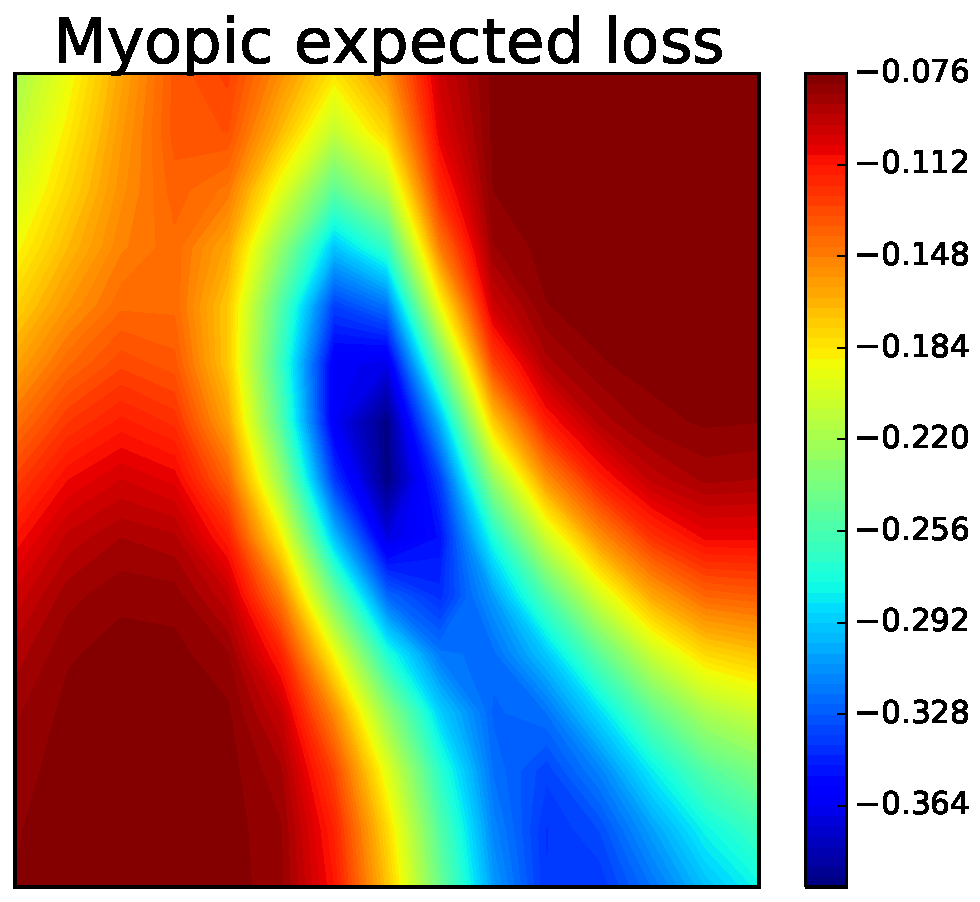
\includegraphics[width=45mm]{1_ahead.pdf}} &
      {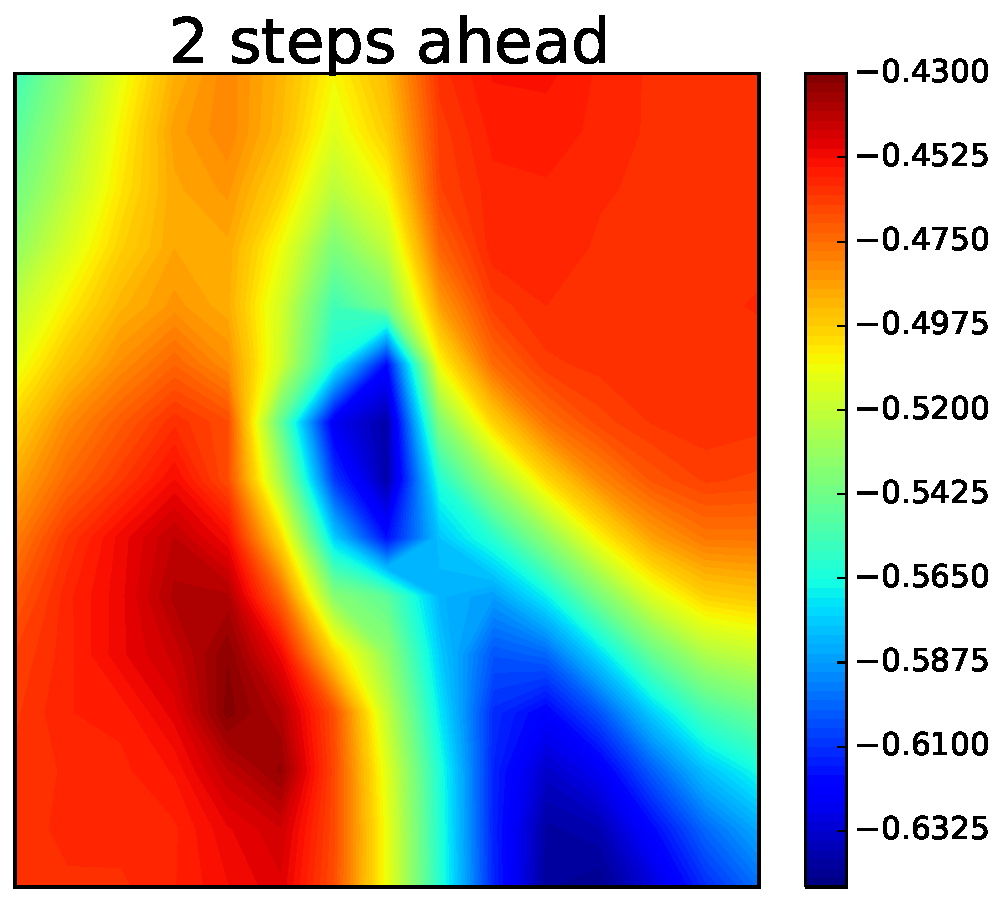
\includegraphics[width=47mm]{2_ahead.pdf}}  &
      {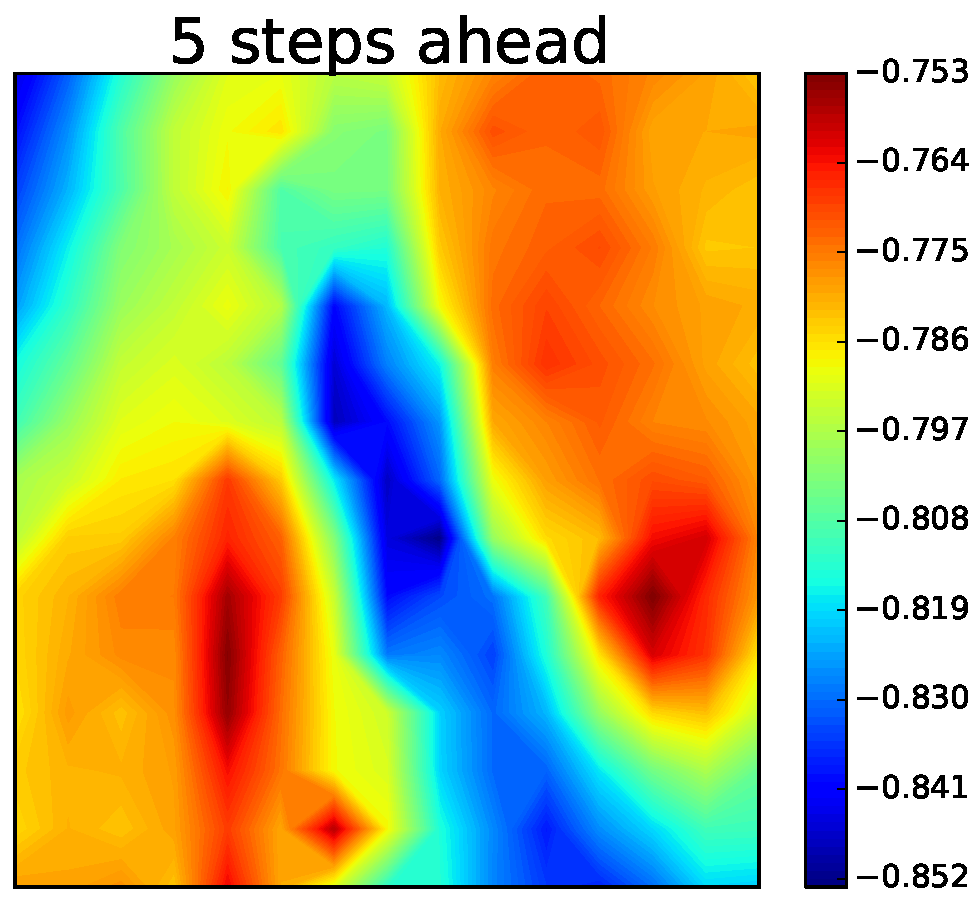
\includegraphics[width=45mm]{5_ahead.pdf}} &
      {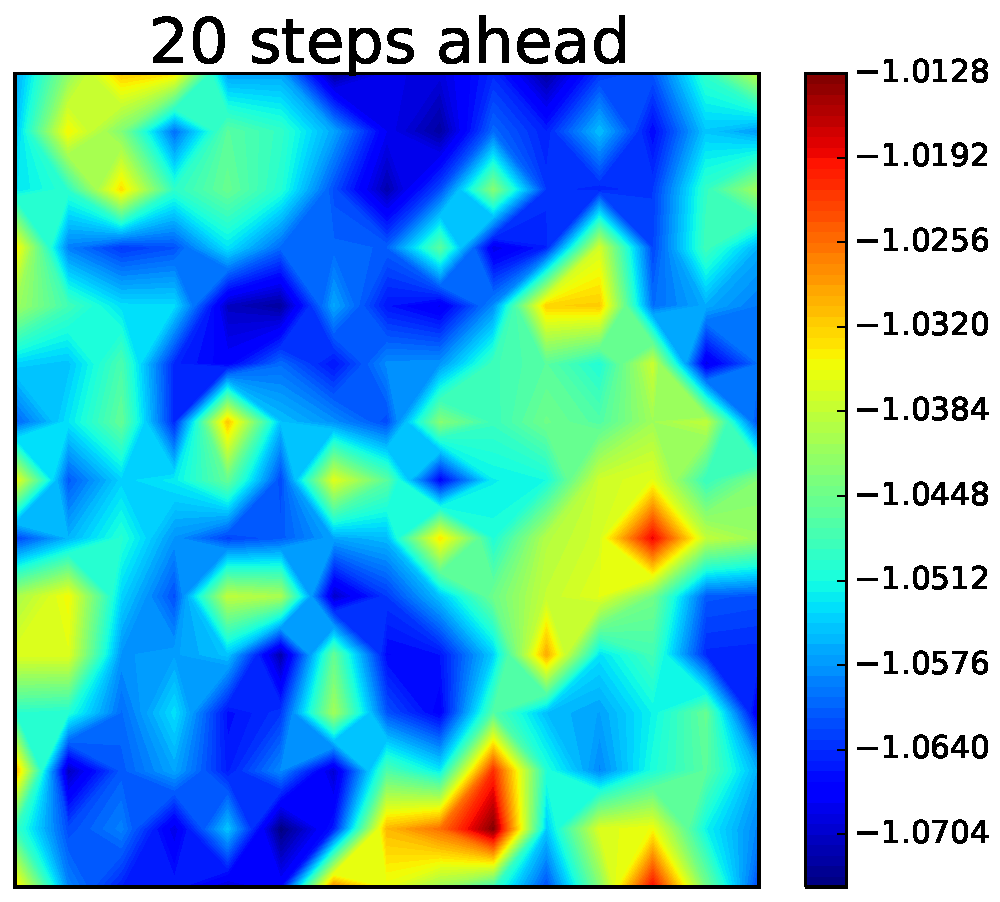
\includegraphics[width=47mm]{20_ahead.pdf}}\\
\end{tabular}\caption{Expected loss for different number of steps ahead in an example with 10 data points and the Six-hump Camel function. }\label{table:n_ahead}
\end{figure}

 \begin{center}
 \textcolor{red}{\textbf{Increasing the number of steps-ahead increased exploration in GLASSES}}
 \end{center}
 

\begin{table}[t!]
\begin{center}
\begin{tabular}{lcccccccc}
\hline
{} &     MPI &     GP-LCB &      EL &    EL-2 &    EL-3 &    EL-5 &  EL-10 &    GLASSES \\
\hline
SinCos  &  0.7147 &  0.6058 &  0.7645 &  \emph{0.8656} &  0.6027 &  0.4881 &  \emph{0.8274} &  \emph{\textbf{0.9000}} \\ 
Cosines           &  0.8637 &  0.8704 &  0.8161 &  \emph{0.8423} &  \emph{0.8118} &  0.7946 &  0.7477 &  \emph{\textbf{0.8722}} \\
Branin              &  0.9854 &  0.9616 &  \textbf{0.9900} &  0.9856 &  0.9673 &  0.9824 &  0.9887 &  0.9811 \\
Sixhumpcamel        &  0.8983 &  \textbf{0.9346} &  0.9299 &  0.9115 &  0.9067 &  0.8970 &  0.9123 &  0.8880 \\
Mccormick           & \textbf{0.9514} &  0.9326 &  0.9055 &  \emph{0.9139} &  \emph{0.9189} &  \emph{0.9283} &  \emph{0.9389} &  \emph{0.9424} \\
Dropwave            &  0.7308 &  0.7413 &  0.7667 &  0.7237 &  0.7555 &  0.7293 &  0.6860 &  \emph{\textbf{0.7740}} \\
%Beale &&& &&&&&\\ 
Powers              &  0.2177 &  0.2167 &  0.2216 &  \emph{0.2428} &  \emph{0.2372} &  \emph{0.2390} &  \emph{0.2339} &  \emph{\textbf{0.3670}} \\
Ackley-2 &  0.8230 &  \textbf{0.8975} &  0.7333 &  0.6382 &  0.5864 &  0.6864 &  0.6293 &  0.7001 \\
Ackley-5  & 0.1832&   0.2082&   0.5473&   \emph{0.6694}&  0.3582&   0.3744&   \emph{\textbf{0.6700}} &  0.4348\\ 
Ackley-10 &  0.9893 &  0.9864 &  0.8178 &   \emph{0.9900} &   \emph{0.9912} &   \emph{\textbf{0.9916}} &   \emph{0.8340} &   \emph{0.8567} \\
Alpine2-2 &  \textbf{0.8628} &  0.8482 &  0.7902 &  0.7467 &  0.5988 &  0.6699 &  0.6393 &  0.7807 \\
Alpine2-5  &  0.5221 &  0.6151 &  \textbf{0.7797} &  0.6740 &  0.6431 &  0.6592 &  0.6747 &  0.7123 \\
\hline
\end{tabular}\caption{Results for the average `gap' measure (5 replicates) across different functions.  EL-k: expect loss with $k$ steps ahead. MPI: maximum probability of improvement. GP-LCB: lower confidence bound criterion. }
\end{center}
\end{table}
 \begin{center}
 \textcolor{red}{\textbf{Non-myopic losses improve the results in practice }}
 \end{center}
 

      \end{block}



      %-- Block 3-2
      \begin{block}{Conclusions and future work}
\begin{itemize}
\item First non-myopic loss that allows taking into account dozens of future evaluations.
\item The loss compares well with current myopic acquisitions.
\item Challenge: making the optimisation of the loss more efficient.
\end{itemize}

      \end{block}

\begin{block}{References}
\begin{itemize}
\item[1] Michael Osborne. Bayesian Gaussian Processes for Sequential Prediction, Optimisation and Quadrature. PhD thesis, University of Oxford, 2010.
\item[2] John P. Cunningham, Philipp Hennig, and Simon Lacoste-Julien. Gaussian probabilities and expectation propagation. arXiv:1111.6832 [stat], Nov 2011. arXiv: 1111.6832.
\item[3] Javier Gonz\'alez, Zhenwen Dai, Philipp Hennig, and Neil D Lawrence. Batch Bayesian optimization via local penalization. arXiv preprint arXiv:1505.08052, 2015.
\end{itemize}

\end{block}

    \end{column}%3

  \end{columns}
\end{frame}
\end{document}
